\documentclass[tikz,border=5mm]{standalone}
\usepackage{tikz}
\usetikzlibrary{positioning, shapes.geometric, shadows, arrows.meta, backgrounds, fit}

\begin{document}

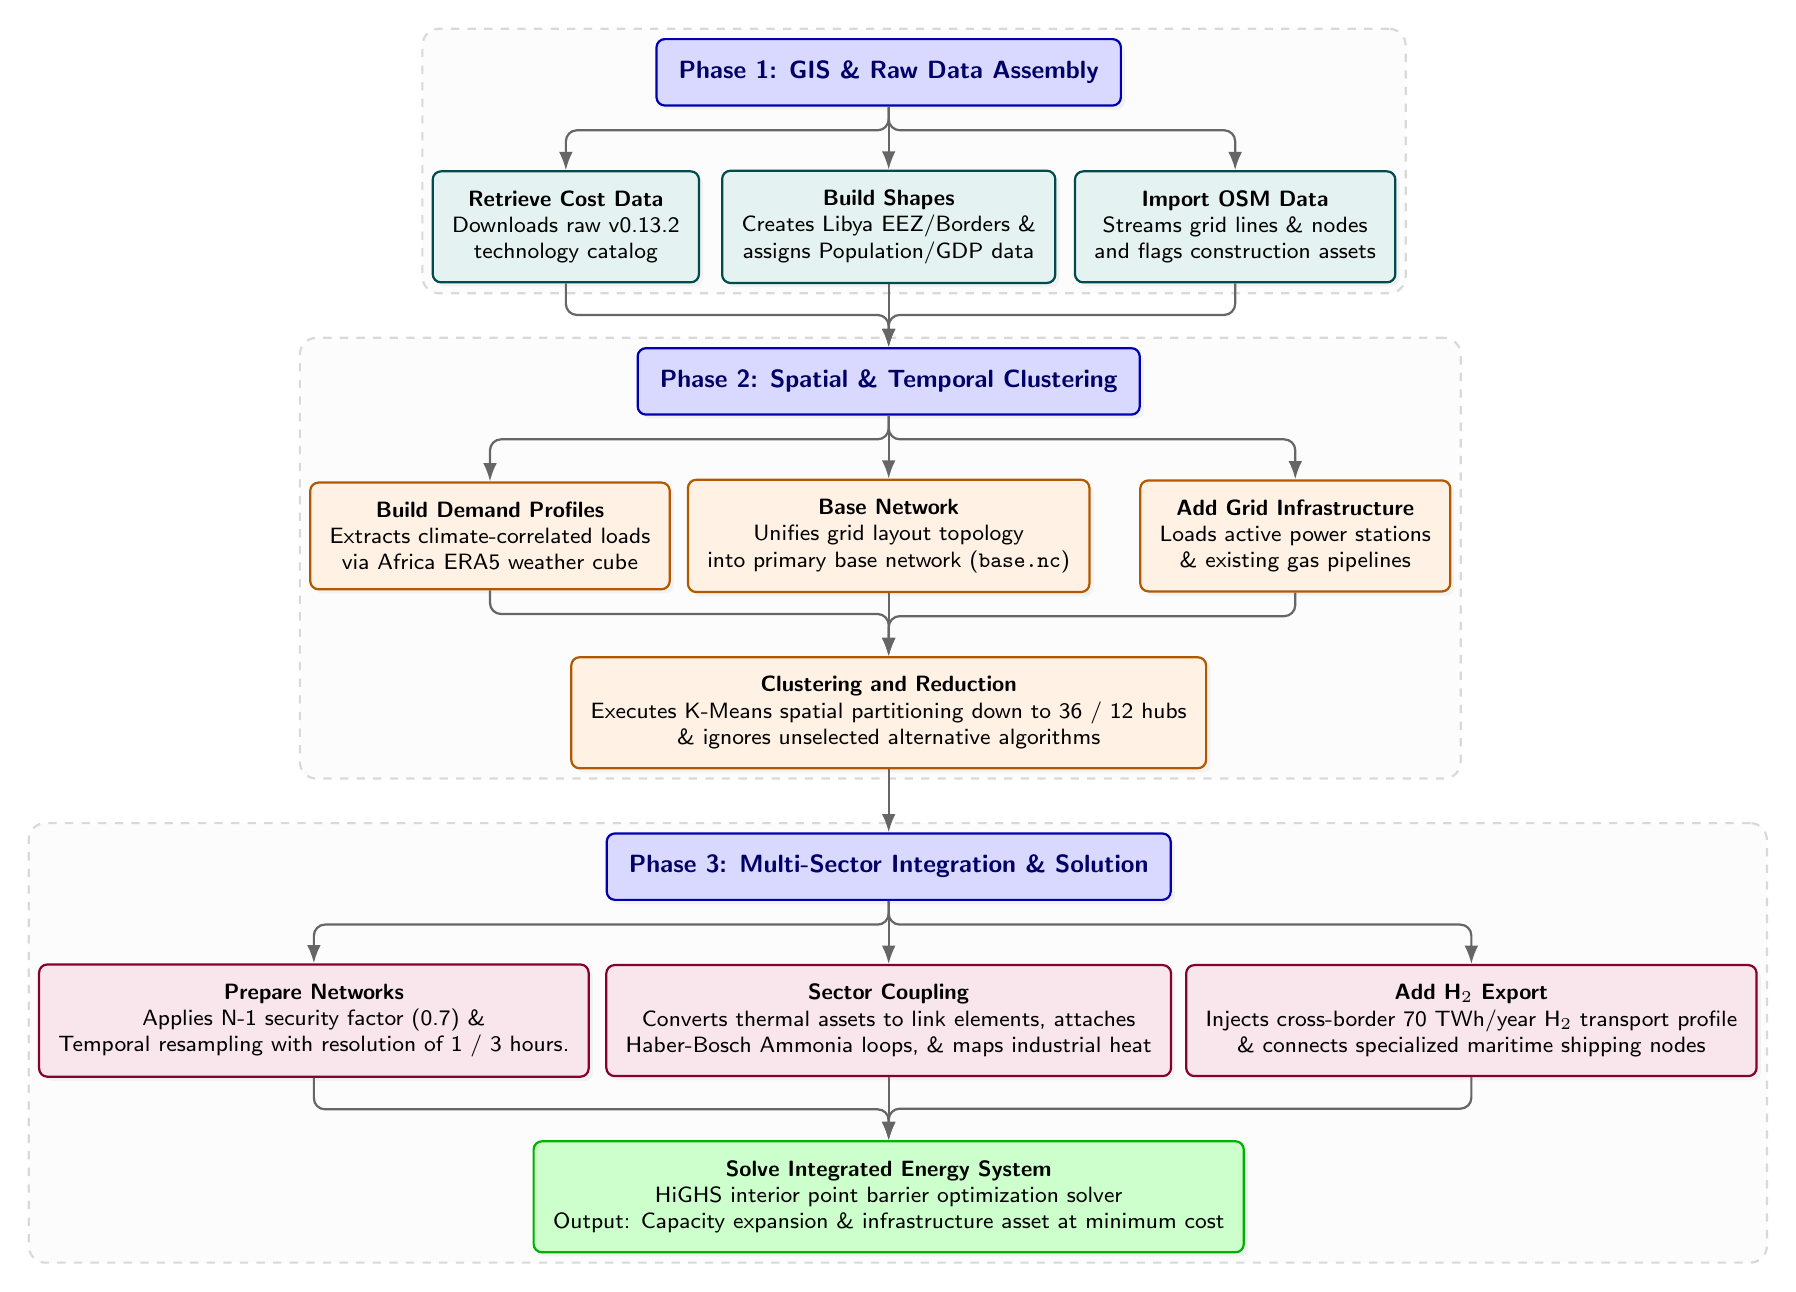
\begin{tikzpicture}[
    % Base node styling
    base/.style={
        draw=gray!50,
        thick,
        rectangle,
        rounded corners=3pt,
        align=center,
        inner sep=7pt,
        font=\sffamily\footnotesize,
        drop shadow={opacity=0.08, shadow xshift=1.5pt, shadow yshift=-1.5pt}
    },
    % Step-specific stylings
    headerNode/.style={
        base,
        draw=blue!70!black,
        fill=blue!15,
        text=blue!40!black,
        font=\sffamily\bfseries\small,
        inner sep=8pt
    },
    gisNode/.style={
        base,
        draw=teal!60!black,
        fill=teal!10,
        text=black
    },
    clusterNode/.style={
        base,
        draw=orange!70!black,
        fill=orange!10,
        text=black
    },
    sectorNode/.style={
        base,
        draw=purple!70!black,
        fill=purple!10,
        text=black
    },
    solveNode/.style={
        base,
        draw=green!70!black,
        fill=green!20,
        text=black
    },
    % Container Grouping Style
    container/.style={
        draw=gray!30,
        dashed,
        thick,
        rounded corners=6pt,
        fill=gray!2
    },
    % Connector line styling
    connector/.style={
        draw=black!60,
        -{Latex[scale=1.0]},
        thick,
        rounded corners=4pt
    }
]

% =====================================================================
% PHASE 1: GEOGRAPHIC & RAW DATA ASSEMBLY (GIS)
% =====================================================================
\node[headerNode] (h1) {Phase 1: GIS \& Raw Data Assembly};

% 1. Place the main central node
\node[gisNode, below=0.8cm of h1] (build_shapes) {
    \textbf{Build Shapes} \\
    Creates Libya EEZ/Borders \& \\
    assigns Population/GDP data
};

% 2. Position left node directly on the horizontal center line of build_shapes
\node[gisNode, left=4.1cm of build_shapes.center, anchor=center] (retrieve_costs) {
    \textbf{Retrieve Cost Data} \\
    Downloads raw v0.13.2 \\
    technology catalog
};

% 3. Position right node directly on the horizontal center line of build_shapes
\node[gisNode, right=4.4cm of build_shapes.center, anchor=center] (download_osm) {
    \textbf{Import OSM Data} \\
    Streams grid lines \& nodes \\
     and flags construction assets
};

% =====================================================================
% PHASE 2: SPATIAL & TEMPORAL DISCRETIZATION
% =====================================================================
\node[headerNode, below=0.8cm of build_shapes] (h2) {Phase 2: Spatial \& Temporal Clustering};

% Horizontal Row Alignment below Header 2
\node[clusterNode, below=0.8cm of h2] (base_network) {
    \textbf{Base Network} \\
    Unifies grid layout topology \\
    into primary base network (\texttt{base.nc})
};

\node[clusterNode, left=2.5cm of base_network, anchor=center] (demand_profiles) {
    \textbf{Build Demand Profiles} \\
    Extracts climate-correlated loads \\
    via Africa ERA5 weather cube
};

\node[clusterNode, right=2.6cm of base_network, anchor=center] (add_elec) {
    \textbf{Add Grid Infrastructure} \\
    Loads active power stations \\
    \& existing gas pipelines
};

\node[clusterNode, below=0.8cm of base_network] (cluster_net) {
    \textbf{Clustering and Reduction} \\
    Executes {K-Means} spatial partitioning down to {36 /  12 hubs} \\
    \& ignores unselected alternative algorithms
};


% =====================================================================
% PHASE 3: SECTOR COUPLING & MATRIC SOLVER
% =====================================================================
\node[headerNode, below=0.8cm of cluster_net] (h3) {Phase 3: Multi-Sector Integration \& Solution};

% Horizontal Row Alignment below Header 3
\node[sectorNode, below=0.8cm of h3] (prep_sector) {
    \textbf{Sector Coupling} \\
    Converts thermal assets to link elements, attaches \\
    Haber-Bosch Ammonia loops, \& maps industrial heat
};

\node[sectorNode, left=3.7cm of prep_sector, anchor=center] (prepare_net) {
    \textbf{Prepare Networks} \\
    Applies N-1 security factor (0.7) \& \\
    {Temporal resampling with resolution of 1 / 3 hours.}
};

\node[sectorNode, right=3.8cm of prep_sector, anchor=center] (add_export) {
    \textbf{Add H$_2$ Export} \\
    Injects cross-border {70 TWh/year} H$_2$ transport profile \\
    \& connects specialized maritime shipping nodes
};

\node[solveNode, below=0.8cm of prep_sector] (highs) {
     \textbf{Solve Integrated Energy System} \\
    HiGHS interior point barrier optimization solver \\
    Output: Capacity expansion \& infrastructure asset at minimum cost 
};

% =====================================================================
% BACKGROUND CONTAINERS
% =====================================================================
\begin{scope}[on background layer]
    \node[container, fit=(h1) (retrieve_costs) (build_shapes) (download_osm)] (box1) {};
    \node[container, fit=(h2) (demand_profiles) (base_network) (add_elec) (cluster_net)] (box2) {};
    \node[container, fit=(h3) (prepare_net) (prep_sector) (add_export) (highs)] (box3) {};
\end{scope}


% =====================================================================
% CONNECTOR PATHS (RECONFIGURED TREE ROUTING)
% =====================================================================

% Phase 1 Connectors
\draw[connector] (h1.south) -- (build_shapes.north);
\draw[connector] (h1.south) -- ++(0,-0.3) -| (retrieve_costs.north);
\draw[connector] (h1.south) -- ++(0,-0.3) -| (download_osm.north);


% Transition Phase 1 to Phase 2 Main Trunk
\draw[connector] (retrieve_costs.south) -- ++(0,-0.4) -| (h2.north);
\draw[connector] (build_shapes.south) -- (h2.north);
\draw[connector] (download_osm.south) -- ++(0,-0.4) -| (h2.north);


% Phase 2 Connectors
\draw[connector] (h2.south) -- (base_network.north);
\draw[connector] (h2.south) -- ++(0,-0.3) -| (demand_profiles.north);
\draw[connector] (h2.south) -- ++(0,-0.3) -| (add_elec.north);

% Convergence to Clustering Node
\draw[connector] (demand_profiles.south) -- ++(0,-0.3) -| (cluster_net.north);
\draw[connector] (base_network.south) -- (cluster_net.north);
\draw[connector] (add_elec.south) -- ++(0,-0.3) -| (cluster_net.north);

% Transition Phase 2 to Phase 3 Main Trunk
\draw[connector] (cluster_net.south) -- (h3.north);

% Phase 3 Connectors
\draw[connector] (h3.south) -- (prep_sector.north);
\draw[connector] (h3.south) -- ++(0,-0.3) -| (prepare_net.north);
\draw[connector] (h3.south) -- ++(0,-0.3) -| (add_export.north);

% Convergence from Row to Final Solver Block
\draw[connector] (prepare_net.south) -- ++(0,-0.4) -| (highs.north);
\draw[connector] (prep_sector.south) -- (highs.north);
\draw[connector] (add_export.south) -- ++(0,-0.4) -| (highs.north);

\end{tikzpicture}
\end{document}
